\documentclass[a4paper,11pt,dvipdfmx]{jsarticle}

\usepackage{bm}
\usepackage[dvipdfmx]{graphicx}
\usepackage[dvipdfmx]{color}
\usepackage{ascmac}
\usepackage{siunitx}
\usepackage{otf}
\pagestyle{plain}
\usepackage{float}
\usepackage[dvipdfmx]{hyperref}
\usepackage{pxjahyper}
\usepackage{here}
\usepackage{titlesec}
\titleformat*{\section}{\LARGE\bfseries}
\titleformat*{\subsection}{\normalsize\bfseries}
\usepackage{url}
\usepackage{comment}
\usepackage[table,xcdraw]{xcolor}
\hypersetup{% hyperrefオプションリスト
setpagesize=false,
 bookmarksnumbered=true,%
 bookmarksopen=true,%
 colorlinks=true,%
 linkcolor=blue,
 citecolor=blue,
}

\begin{document}


\subsection{エネルギー較正}
本節は得られたデータからエネルギー校正を行うことを目的とする。また較正されたエネルギースペクトルの分析も行う。本研究でのデータ解析は主に、CERN(欧州原子核研究機関)が開発する解析フレームワークROOTを用いて行った。

\subsubsection{理論値の導出}
エネルギー較正に用いるため、各角度での散乱陽子のエネルギー理論値を求める。
散乱が弾性散乱であると仮定する。入射陽子がターゲット原子核のクーロンポテンシャルの働かない十分遠方から飛んでくるとすると、エネルギー保存則と運動量保存則より以下の式が求められる。


\begin{equation}
\centering
\large
  E = \left( \frac{\cos\theta+\sqrt{\cos\theta^2+A^2-1}}{A+1} \right)^2 E_0
  \label{scatter}
\end{equation}

\vspace*{2mm}

\begin{center}
\begin{small}
  $\it{E}$:散乱後の陽子のエネルギー $E_0$:入射陽子のエネルギー\\
  $\theta$:実験室系の散乱角度[$^\circ$] A:ターゲット原子の質量数
\end{small}
\end{center} 

\vspace*{5mm}
\noindent
式\ref{scatter}より得られた、各ターゲット原子核に散乱された陽子(入射エネルギー:3MeV)のエネルギーの角度依存性を図\ref{angleE}に示す。

\begin{figure}[H]
\centering
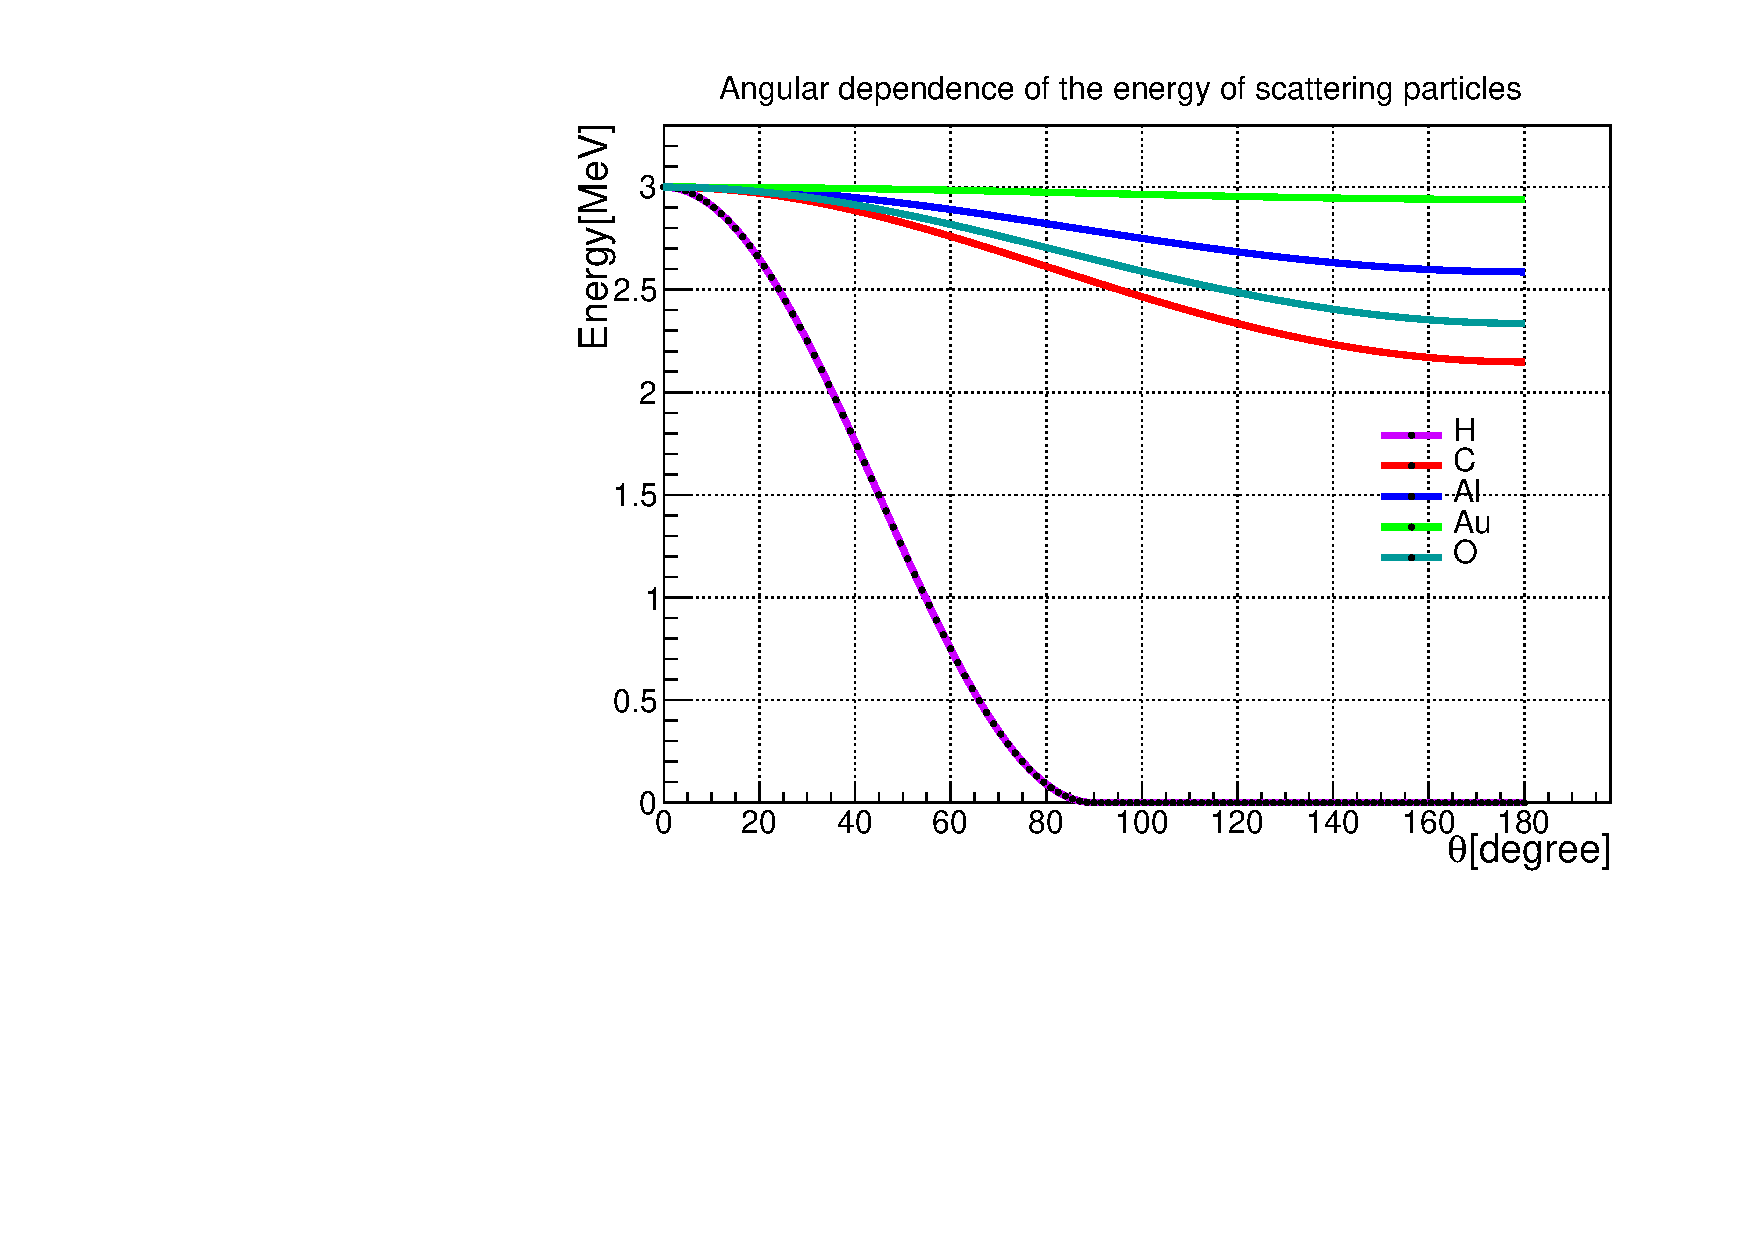
\includegraphics[width=120mm]{picture/cali/protonE.pdf}
\caption{散乱陽子のエネルギーの角度依存性}
\label{angleE}
\end{figure}

\newpage
またターゲットは厚さを持ち、入射粒子や反跳粒子は荷電粒子であることから、Bethe-Blochの式に従いエネルギー損失を起こす。陽子におけるBethe-Blochの式を以下に示す。

\vspace*{2mm}

\begin{equation}
\centering
\large
 -\frac{1}{\rho}\frac{dE}{dx} = \frac{4\pi{N_A}}{{m_e}c^2}{\left( \frac{e^2}{4\pi\varepsilon_0}\right)}^2\frac{Z}{A}\frac{1}{\beta^2}\left[\ln{\left(\frac{2m_ec^2\beta^2}{I(1-\beta^2)} \right)-\beta^2}\right]
  \label{BB}
\end{equation}

\vspace*{2mm}

\begin{center}
\begin{small}
 $\rho$:ターゲットの密度[kg/m$^3$] $N_A$:アボガドロ数[/mol] \\
 \vspace*{1mm}
  $m_e$:電子の質量[eV/c$^2$] c:光速[m/s] \\
  %\vspace*{0.5mm}
  e:電気素量[C] $\varepsilon_0$:真空の誘電率 \\
  \vspace*{0.5mm}
  Z:ターゲットの原子番号 $\beta=\frac{v}{c}:陽子の相対速度$ \\
 %\vspace*{0.3mm}
  $I\simeq16\cdot{Z^{0.9}}$:平均イオン化ポテンシャル[eV]
\end{small}
\end{center}

\noindent
以上の2つの式を用いてエネルギーの理論値を求めた。次節ではその値から予想されるエネルギースペクトルとの比較を行う。\\

\subsubsection{エネルギースペクトルの分析}
各角度でのエネルギースペクトルの分析を行なった。エネルギーの測定値は正規分布に従うと考えられるので、各ターゲット原子核に散乱された陽子はエネルギースペクトル上にピークとして現れる。各ピークとエネルギー理論値との対応を考えた。ここではいくつかの例を示す。\\

\begin{itemize}
  \item 標的が金箔のとき\mbox{}\\
  金原子核を標的としたときのエネルギースペクトルには、総じて1つのピークが見られた。図\ref{angleE}より、金原子核に散乱された陽子のエネルギーは角度による変化が小さいことが分かる。本研究でもその傾向が見られたので、散乱陽子のピークだと結論づけた。30$^{\circ}$と140$^{\circ}$におけるスペクトルをそれぞれ図\ref{Au30}、図\ref{Au140}に示す。
  
   \begin{figure}[H]
    \begin{tabular}{cc}
      \begin{minipage}[t]{0.45\hsize}
        \centering
        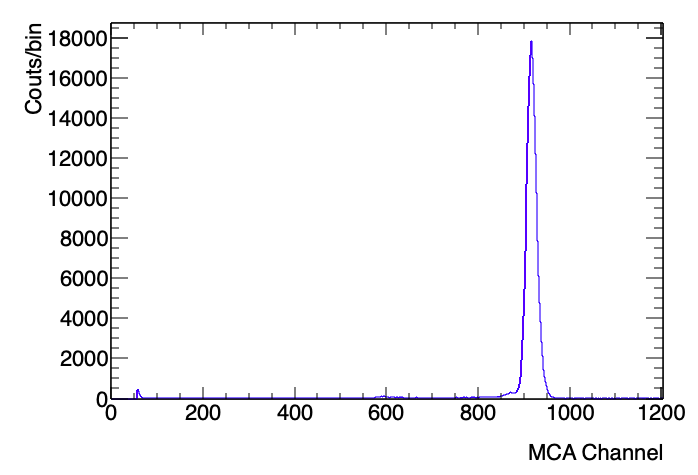
\includegraphics[width=60mm,height=42mm]{picture/cali/Au30.png}
        \caption{30$^{\circ}$におけるスペクトル(MCA)}
        \label{Au30}
      \end{minipage} &
      \begin{minipage}[t]{0.45\hsize}
        \centering
        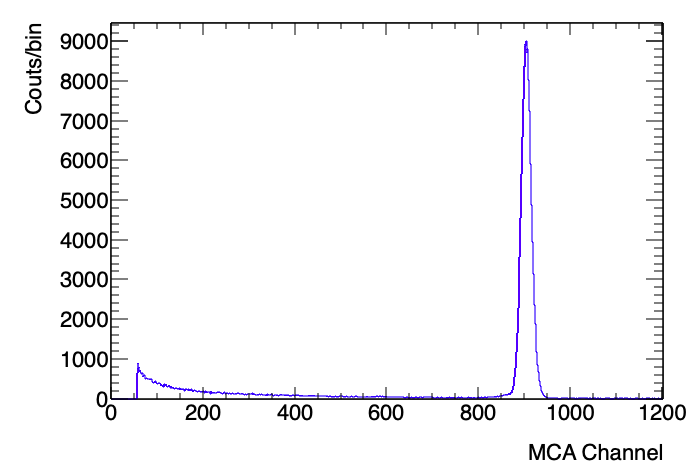
\includegraphics[width=60mm,height=42mm]{picture/cali/Au140.png}
        \caption{140$^{\circ}$におけるスペクトル(MCA)}
        \label{Au140}
      \end{minipage}
    \end{tabular}
  \end{figure}
  
  \item 標的がポリエチレンのとき(低角度)\mbox{}\\
  ポリエチレンの組成式は $(\text{CH}_2)_n$ で表される。図\ref{angleE}より、低角度($\theta\leq90^{\circ}$)では炭素原子核に散乱された陽子のエネルギーは水素原子核によるものよりも大きく、角度と共にその差は大きくなっていく。従って角度が大きくなるにつれて分離されたピークが見られると予想でき、そのような様子が見られた。[図\ref{PE30}] [図\ref{PE60}]\\
  
   \begin{figure}[H]
    \begin{tabular}{cc}
      \begin{minipage}[t]{0.45\hsize}
        \centering
        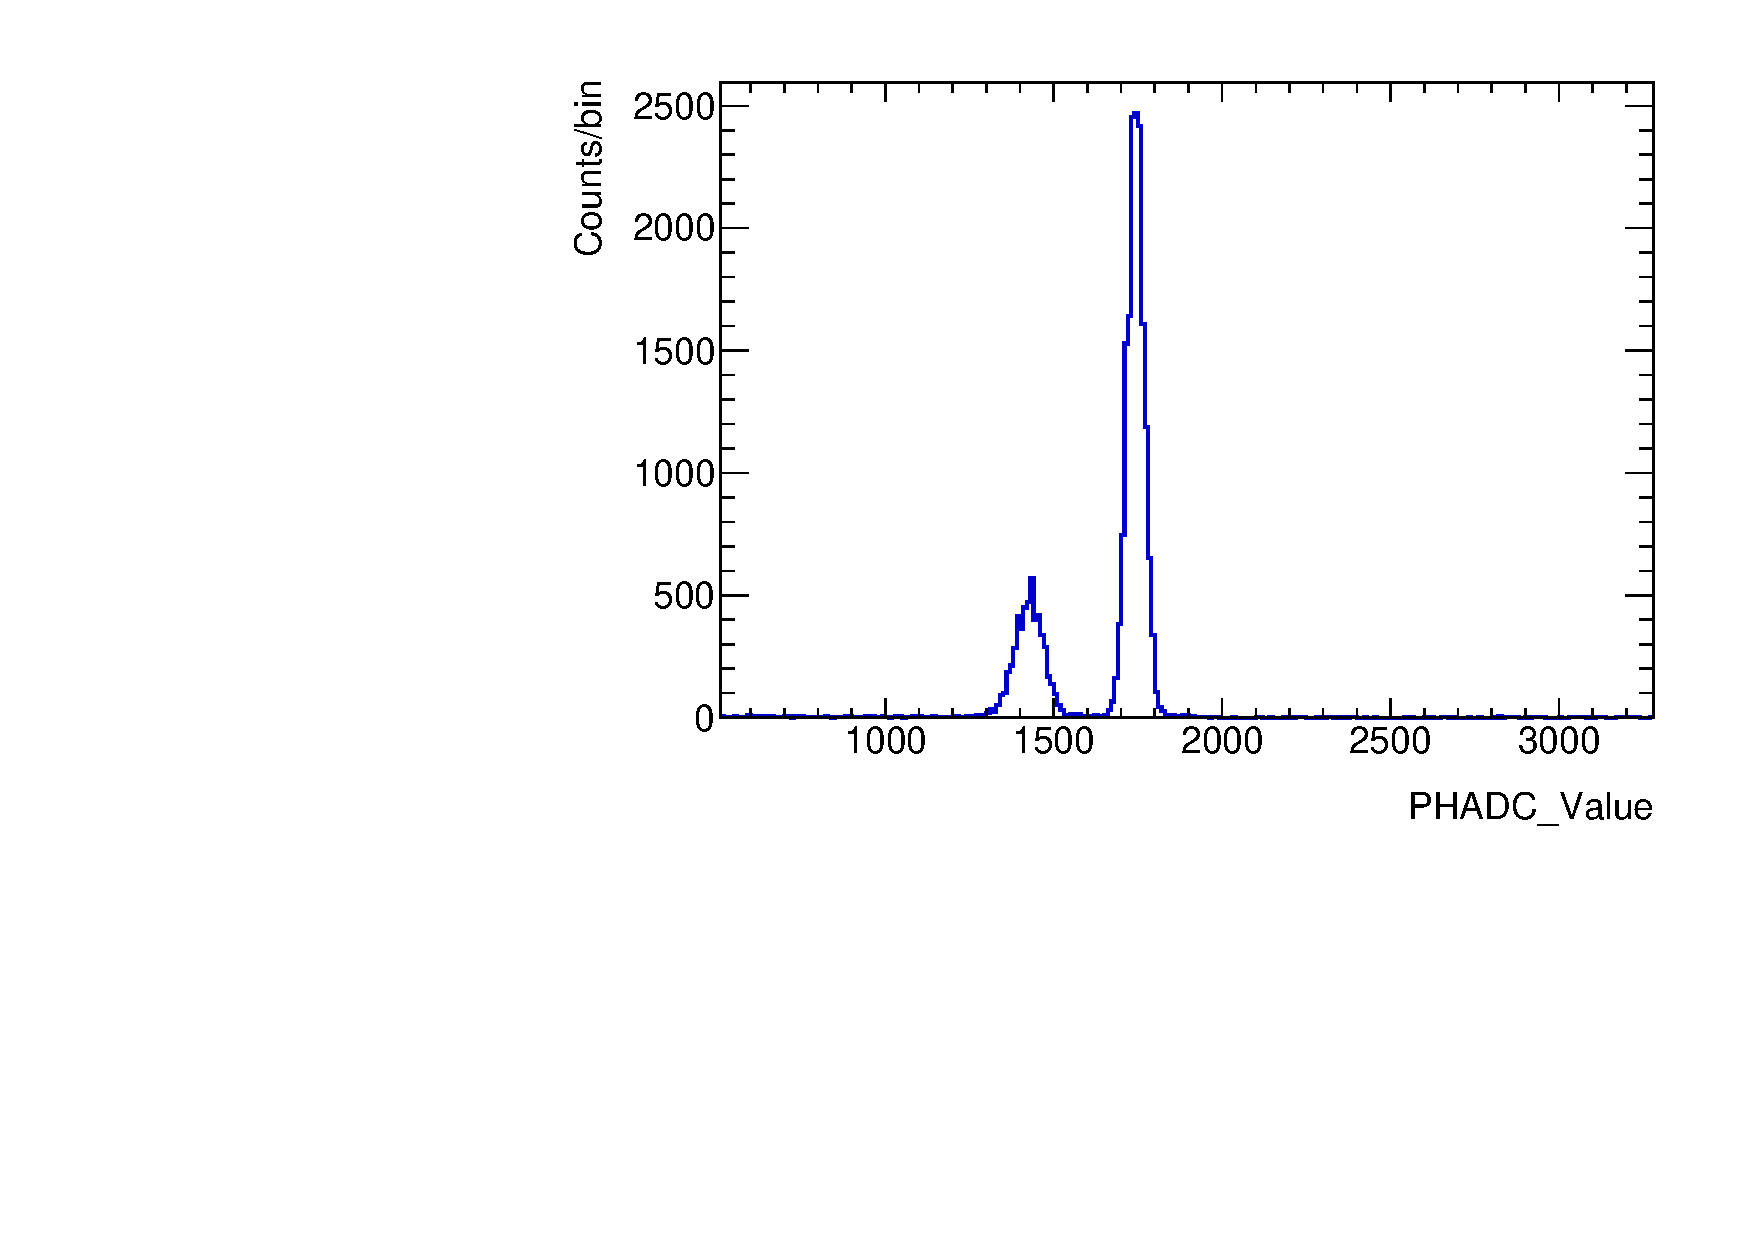
\includegraphics[width=60mm,height=42mm]{picture/cali/adc30.pdf}
        \caption{30$^{\circ}$におけるスペクトル(ADC)}
        \label{PE30}
      \end{minipage} &
      \begin{minipage}[t]{0.45\hsize}
        \centering
        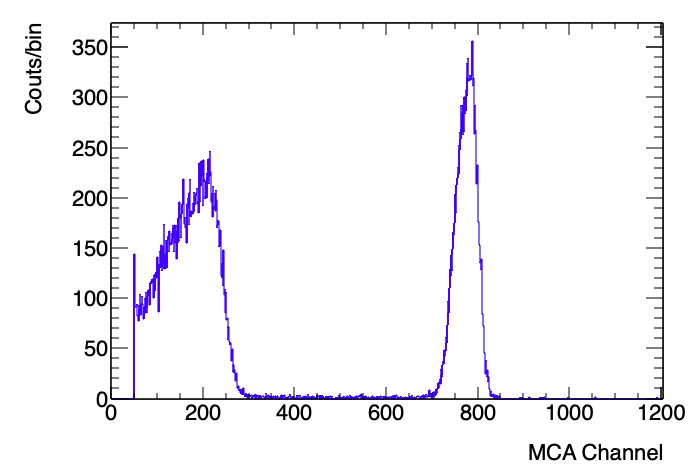
\includegraphics[width=60mm,height=42mm]{picture/cali/PE60.png}
        \caption{60$^{\circ}$におけるスペクトル(MCA)}
        \label{PE60}
      \end{minipage}
    \end{tabular}
  \end{figure}
  
  60$^{\circ}$のエネルギースペクトルにおいて水素原子核由来のピークはガウス関数の低エネルギー側が潰れたような形をしている。これは粒子のエネルギーが低いためMCAのペデスタルにかかってしまっているからであると考えられる。\\
  
  
  \item 標的がポリエチレンのとき(大角度)\mbox{}\\
  エネルギー保存則と運動量保存則より、水素原子核に衝突した陽子と反跳水素原子核は、大角度($\theta>90^{\circ}$)には散乱されない。従って、炭素原子核に散乱された陽子のピークのみが見られると予想できる。
  
\begin{figure}[H]
\centering
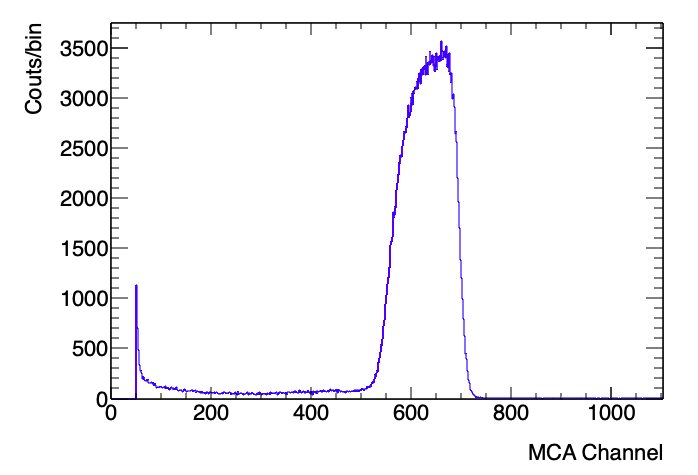
\includegraphics[width=80mm]{picture/cali/PE140.png}
\caption{140$^{\circ}$におけるスペクトル(MCA)}
\label{PE140}
\end{figure}

図\ref{PE140}は140$^{\circ}$におけるエネルギースペクトルである。大角度においてはこのような、ガウシアンに比べてエネルギー分布が広がった形のピークが見られた。これは陽子が入射してから検出器に到達するまでの間の経路差によるものであると考えられる。大角度の散乱では、散乱イベントが発生したターゲット内の位置によってエネルギー損失量に大きな差が生じる。表\ref{Edepo}に30$^{\circ}と140^{\circ}$における、経路の差によって生じるエネルギーの差の最大値を示す。大きな角度で散乱された粒子はターゲット内を進む距離が大きく異なるものが観測されるので、エネルギー分布が図\ref{PE140}のようになると推測される。\\

\begin{table}[h]
\centering
\caption{経路の差によるエネルギーの差}
\begin{tabular}{cccc} \hline
  角度 [$^\circ$] & 最大エネルギー [MeV] & 最小エネルギー [MeV] & エネルギー差 [MeV] \\ \hline
  30 & 2.72 & 2.67 & 0.05 \\ 
  140 &  2.23 & 1.75 & 0.48 \\ \hline
  \label{Edepo}
  \end{tabular}
  \centering
\end{table}

%大きな角度で散乱された粒子はターゲット内を進む距離が大きく異なるものが観測されるので、エネルギー分布が図\ref{PE140}のようになると推測される。

\vspace*{8mm}

\begin{figure}[H]
\centering
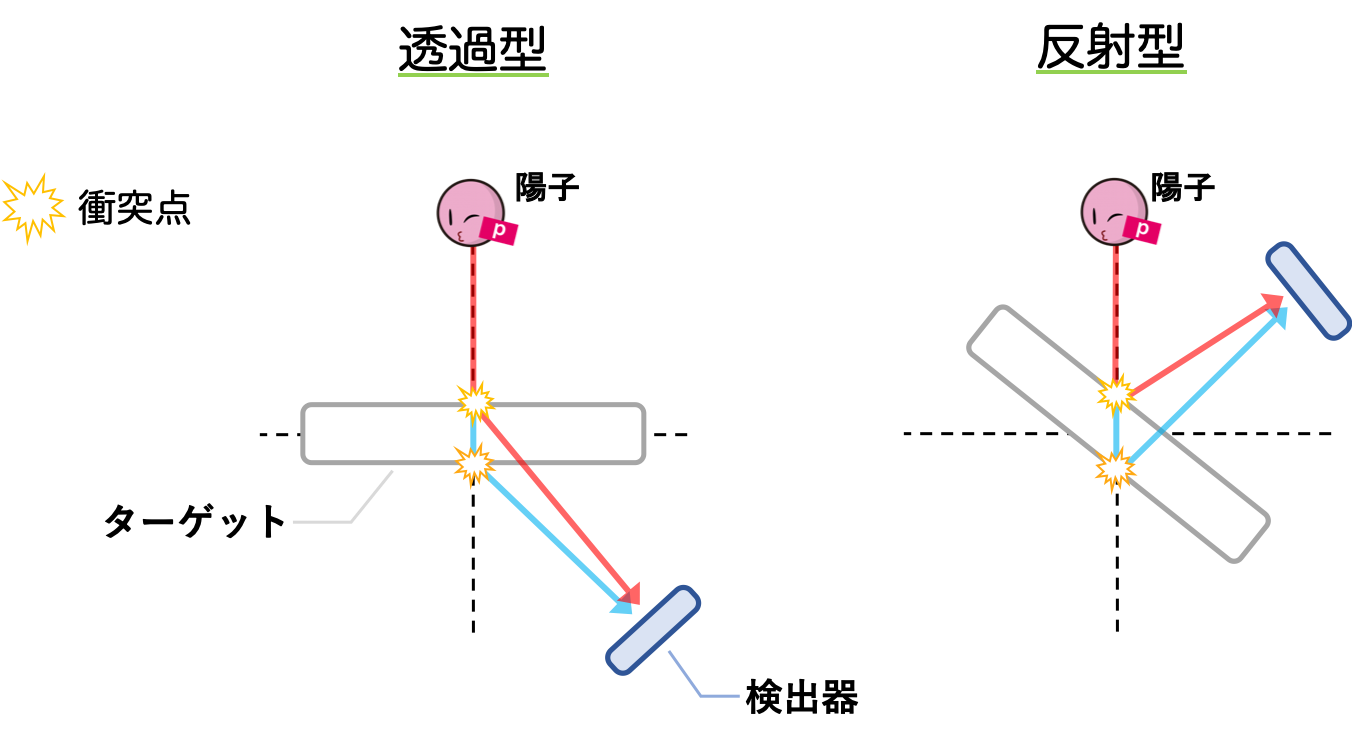
\includegraphics[width=140mm]{picture/cali/d.png}
\caption{散乱角度による経路差 \protect \footnotemark}
\label{dis}
\end{figure}

\footnotetext{陽子イラストはひっぐすたんHPより\\ \url{https://higgstan.com}}

\end{itemize}

\newpage
\subsubsection{較正曲線}
本節では、前節で行ったエネルギースペクトルの分析の結果からエネルギー較正を行う。表\ref{ch1cali}、表\ref{ch2cali}、表\ref{mcacali}にエネルギー較正に用いたデータを示す。各ピークをガウシアンでフィッティングし、Mean値をエネルギー理論値と対応させた。

\begin{table}[h]
\centering
\caption{PHADCのchannel1のエネルギー較正}
\begin{tabular}{cccc} \hline
  ターゲット原子核 & 角度 [$^\circ$] & 理論値 [keV] & PHADC channel \\ \hline
  H & 50 & 1188 & 758.2 \\ 
  C & 50 & 2775 & 1814 \\ 
  C & 60 & 2569 & 1738.72 \\ \hline
  \label{ch1cali}
  \end{tabular}
  \centering
\end{table}
\begin{table}[h]
\centering
\caption{PHADCのchannel2のエネルギー較正}
\begin{tabular}{cccc} \hline
  ターゲット原子核 & 角度 [$^\circ$] & 理論値 [keV] & PHADC channel \\ \hline
  H & 30 & 2113.79 & 1426.89 \\ 
  H & 40 & 1598.55 & 1155 \\ 
  C & 30 & 2801.24 & 1743.61 \\ 
  C & 60 & 2569.32 & 1611 \\ \hline
  \label{ch2cali}
  \end{tabular}
  \centering
\end{table}

   \begin{figure}[H]
    \begin{tabular}{cc}
      \begin{minipage}[t]{0.47\hsize}
        \centering
        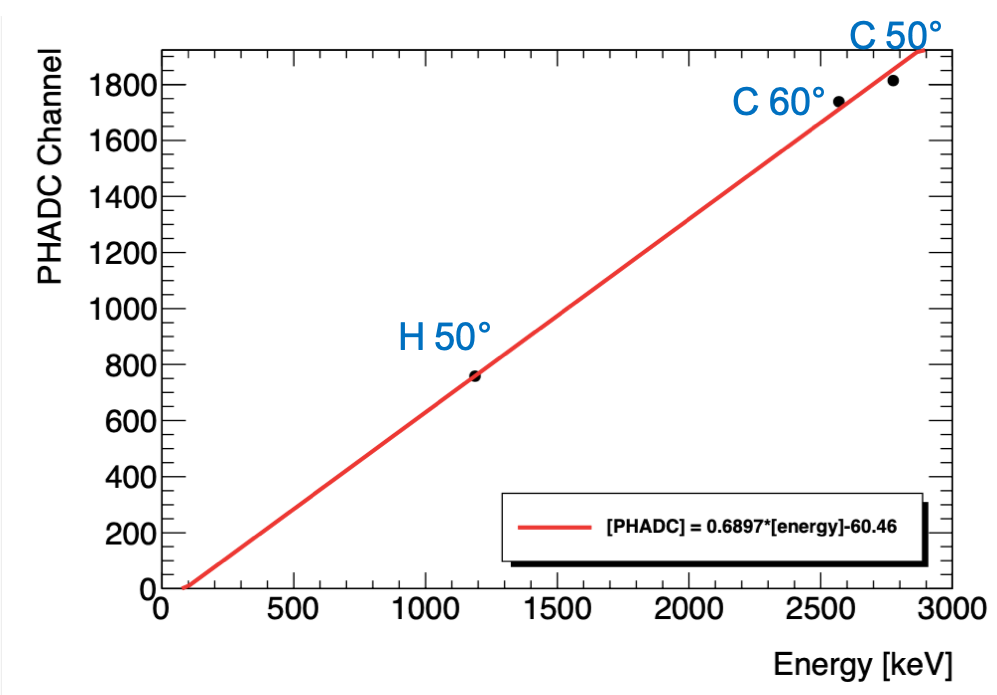
\includegraphics[width=70mm]{picture/cali/calich1.png}
        \caption{PHADC channel1の較正直線}
        \label{ch1line}
      \end{minipage} &
      \begin{minipage}[t]{0.45\hsize}
        \centering
        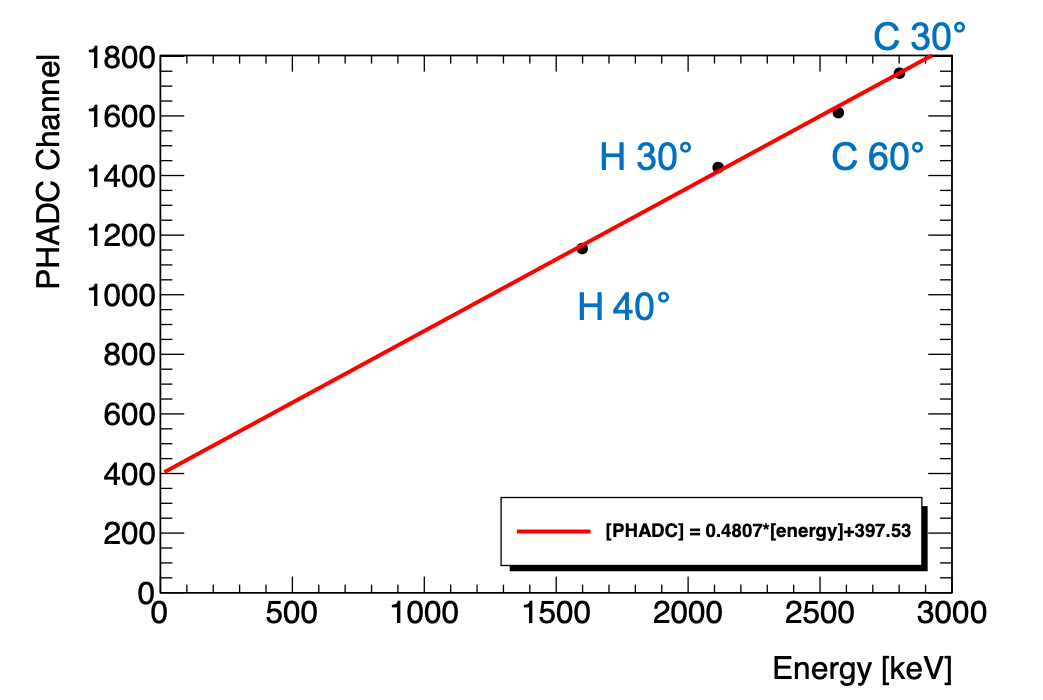
\includegraphics[width=70mm,height=49mm]{picture/cali/calich2.png}
        \caption{PHADC channel2の較正直線}
        \label{ch2line}
      \end{minipage}
    \end{tabular}
  \end{figure}

\vspace{2mm}

\noindent  
\begin{center}
channel1 : Energy [keV] = 1.45 $\times$ PHADC\_channel + 87.66 \\
channel2 : Energy [keV] = 2.08 $\times$ PHADC\_channel - 826.98
\end{center} 

\begin{table}[t]
\centering
\caption{MCAのエネルギー較正}
\begin{tabular}{cccc} \hline
  ターゲット原子核 & 角度 [$^\circ$] & 理論値 [keV] & MCA channel \\ \hline
  Au & 30 & 2981.71 & 916.86 \\ 
  Au & 80 & 2957.91 & 911.10 \\ 
  Au & 130 & 2935.97 & 905.39 \\ 
  C & 40 & 2739.97 & 831.72 \\ 
  H & 70 & 332.08 & 95.66 \\ \hline
  \label{mcacali}
  \end{tabular}
  \centering
\end{table}

\begin{figure}[H]
\centering
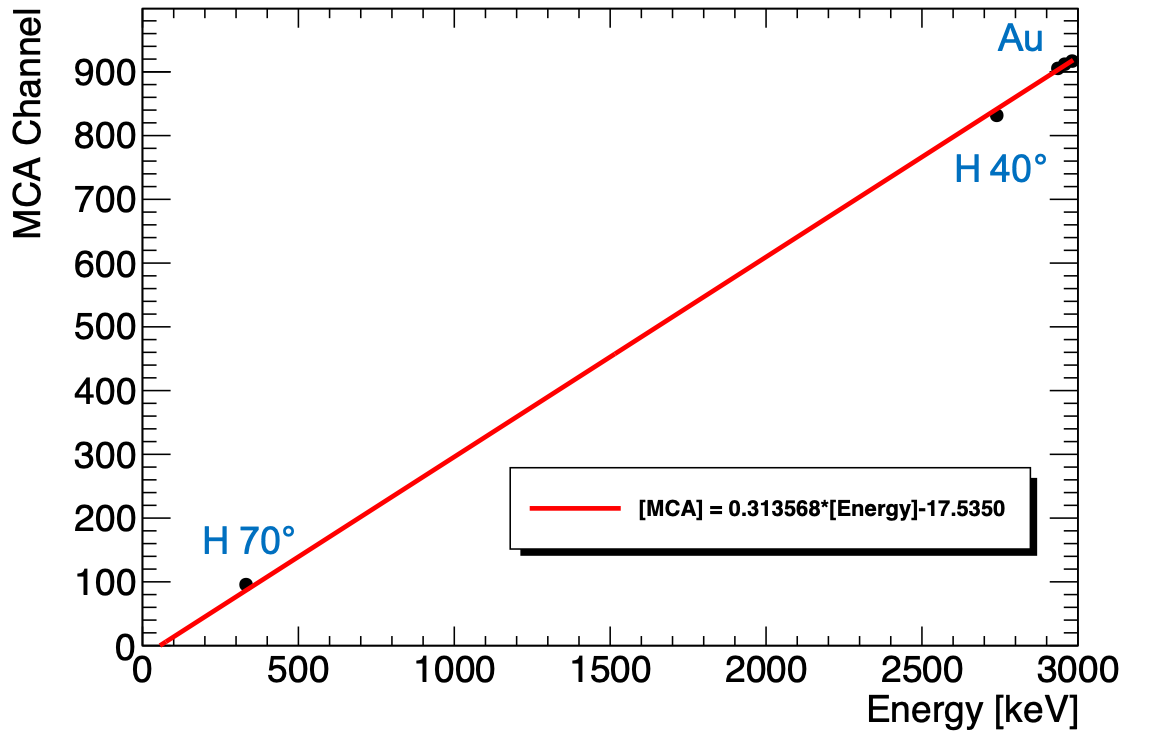
\includegraphics[width=90mm]{picture/cali/mca_cali.png}
\caption{MCAの較正直線}
\label{mca_cali}
Energy [keV] = 3.19 $\times$ MCA\_channel + 55.92
\end{figure}

以上のようにしてエネルギー較正を行った。以降の解析ではここで行った較正データを用いる。

\vspace*{5mm}

\subsubsection{バックグラウンドの考察}
本実験では、期待されていない事象による信号も観測された。本節ではその原因について考察する。以下の図\ref{PE40_BG}に散乱角度40$^\circ$におけるエネルギースペクトルを示す(標的はポリエチレン)。
p-p散乱によるガウスピークが見られなくなるほどのバックグラウンドが観測された。二次電子抑制管の40$^\circ$と50$^\circ$の間にある穴をなべ頭ネジで埋めたことによる影響であると昨年までは結論づけていたため、本年度は皿頭のものを用いてバックグラウンドの排除を試みたが有意な差は得られなかった。

   \begin{figure}[H]
    \begin{tabular}{cc}
      \begin{minipage}[t]{0.47\hsize}
        \centering
        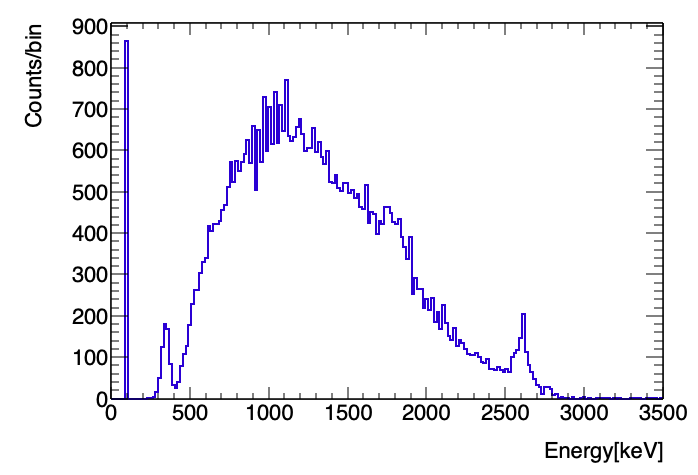
\includegraphics[width=70mm]{picture/cali/PE40_BG.png}
        \caption{40$^\circ$におけるスペクトル(ADC)}
        \label{PE40_BG}
      \end{minipage} &
      \begin{minipage}[t]{0.45\hsize}
        \centering
        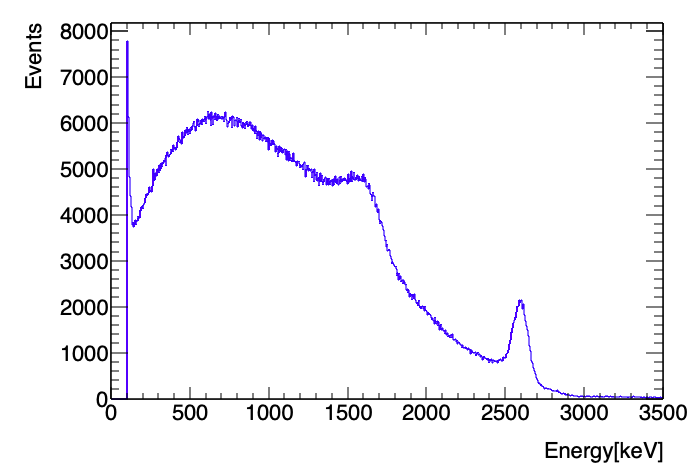
\includegraphics[width=70mm]{picture/cali/PE40_BG2.png}
        \caption{40$^\circ$におけるスペクトル(MCA)}
        \label{PE40_BG2}
      \end{minipage}
    \end{tabular}
  \end{figure}

   \begin{figure}[H]
    \begin{tabular}{cc}
      \begin{minipage}[t]{0.47\hsize}
        \centering
        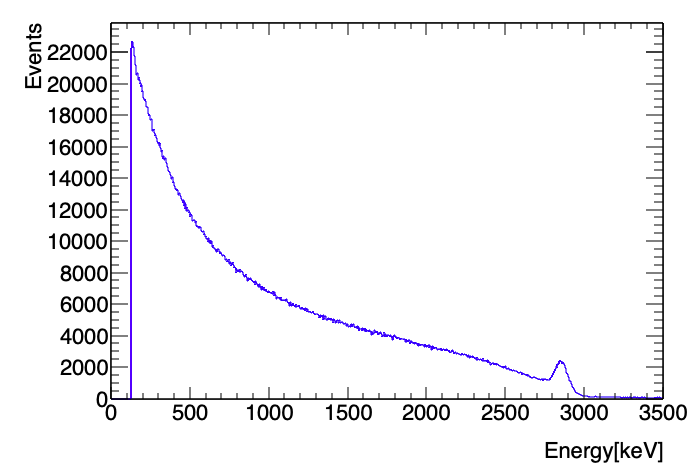
\includegraphics[width=70mm]{picture/cali/AU110_BG.png}
        \caption{110$^\circ$におけるスペクトル(MCA)}
        \label{AU110_BG}
      \end{minipage} &
      \begin{minipage}[t]{0.45\hsize}
        \centering
        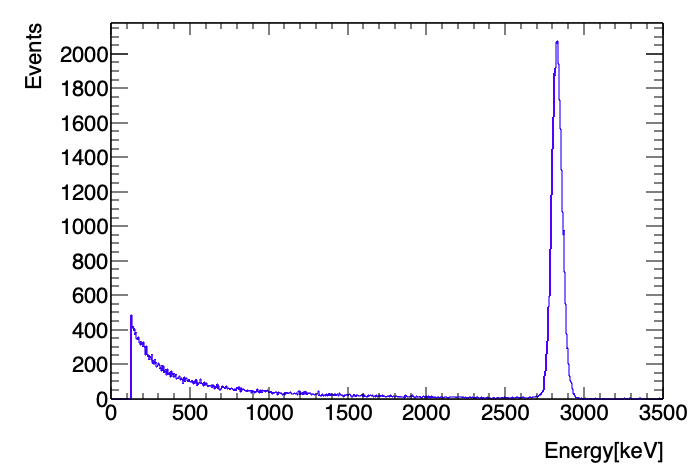
\includegraphics[width=70mm,height=49mm]{picture/cali/AU130_BG.png}
        \caption{130$^\circ$におけるスペクトル(MCA)}
        \label{AU130_BG}
      \end{minipage}
    \end{tabular}
  \end{figure}

\noindent
また100$^\circ\sim120^\circ$の散乱において図\ref{AU110_BG}のような分布も見られた。これはビームストッパーの位置が悪く、陽子を反射してしまったものだと考えられる。130$^\circ$度以上では大幅にバックグラウンドが減少したが、これは検出器がターゲットホルダーの影に隠れたことが原因であると推測される。[図\ref{AU130_BG}]\\

最後に、低角度で見られた期待されなかったピークについて説明する。図\ref{AU20_nazo}のようなピークが金を標的としたときの20$^\circ$、30$^\circ$、ポリエチレンを用いたときの20$^\circ$に見られた。ただし40$^\circ$やポリエチレンのときの30$^\circ$は他の信号に埋れてしまって見えていないと考えられる。
これらのピークの候補としては、反跳された金や炭素の原子核が挙げられる。しかし反跳粒子の散乱断面積は重心系での角度を$\varphi$とすると$\frac{1}{(\cos {\varphi)^3}}$に比例するため\cite{ion}、90度に近づくにつれてより明確にピークが見られるはずである。これらより、反跳原子核によるものではないと結論づけた。

   \begin{figure}[H]
    \begin{tabular}{cc}
      \begin{minipage}[t]{0.47\hsize}
        \centering
        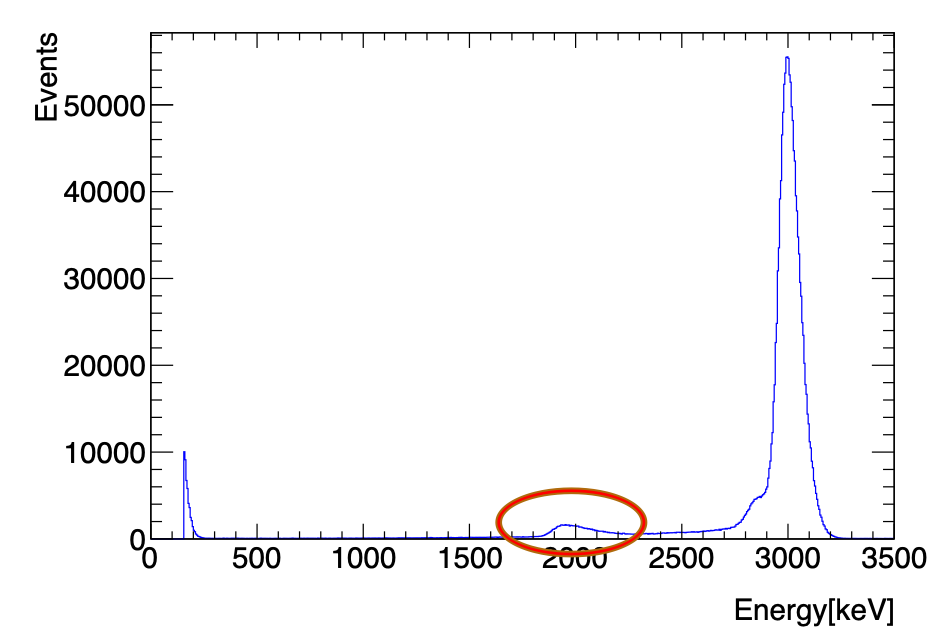
\includegraphics[width=70mm]{picture/cali/AU20_nazo.png}
        \caption{20$^\circ$におけるスペクトル(MCA)}
        \label{AU20_nazo}
      \end{minipage} &
      \begin{minipage}[t]{0.45\hsize}
        \centering
        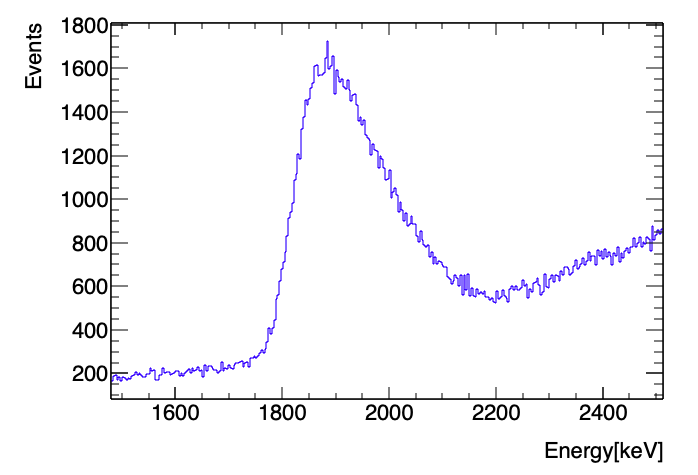
\includegraphics[width=70mm]{picture/cali/AU20_nazo2.png}
        \caption{図\ref{AU20_nazo}を拡大したもの}
        \label{AU20_nazo2}
      \end{minipage}
    \end{tabular}
  \end{figure}
  
\begin{figure}[H]
\centering
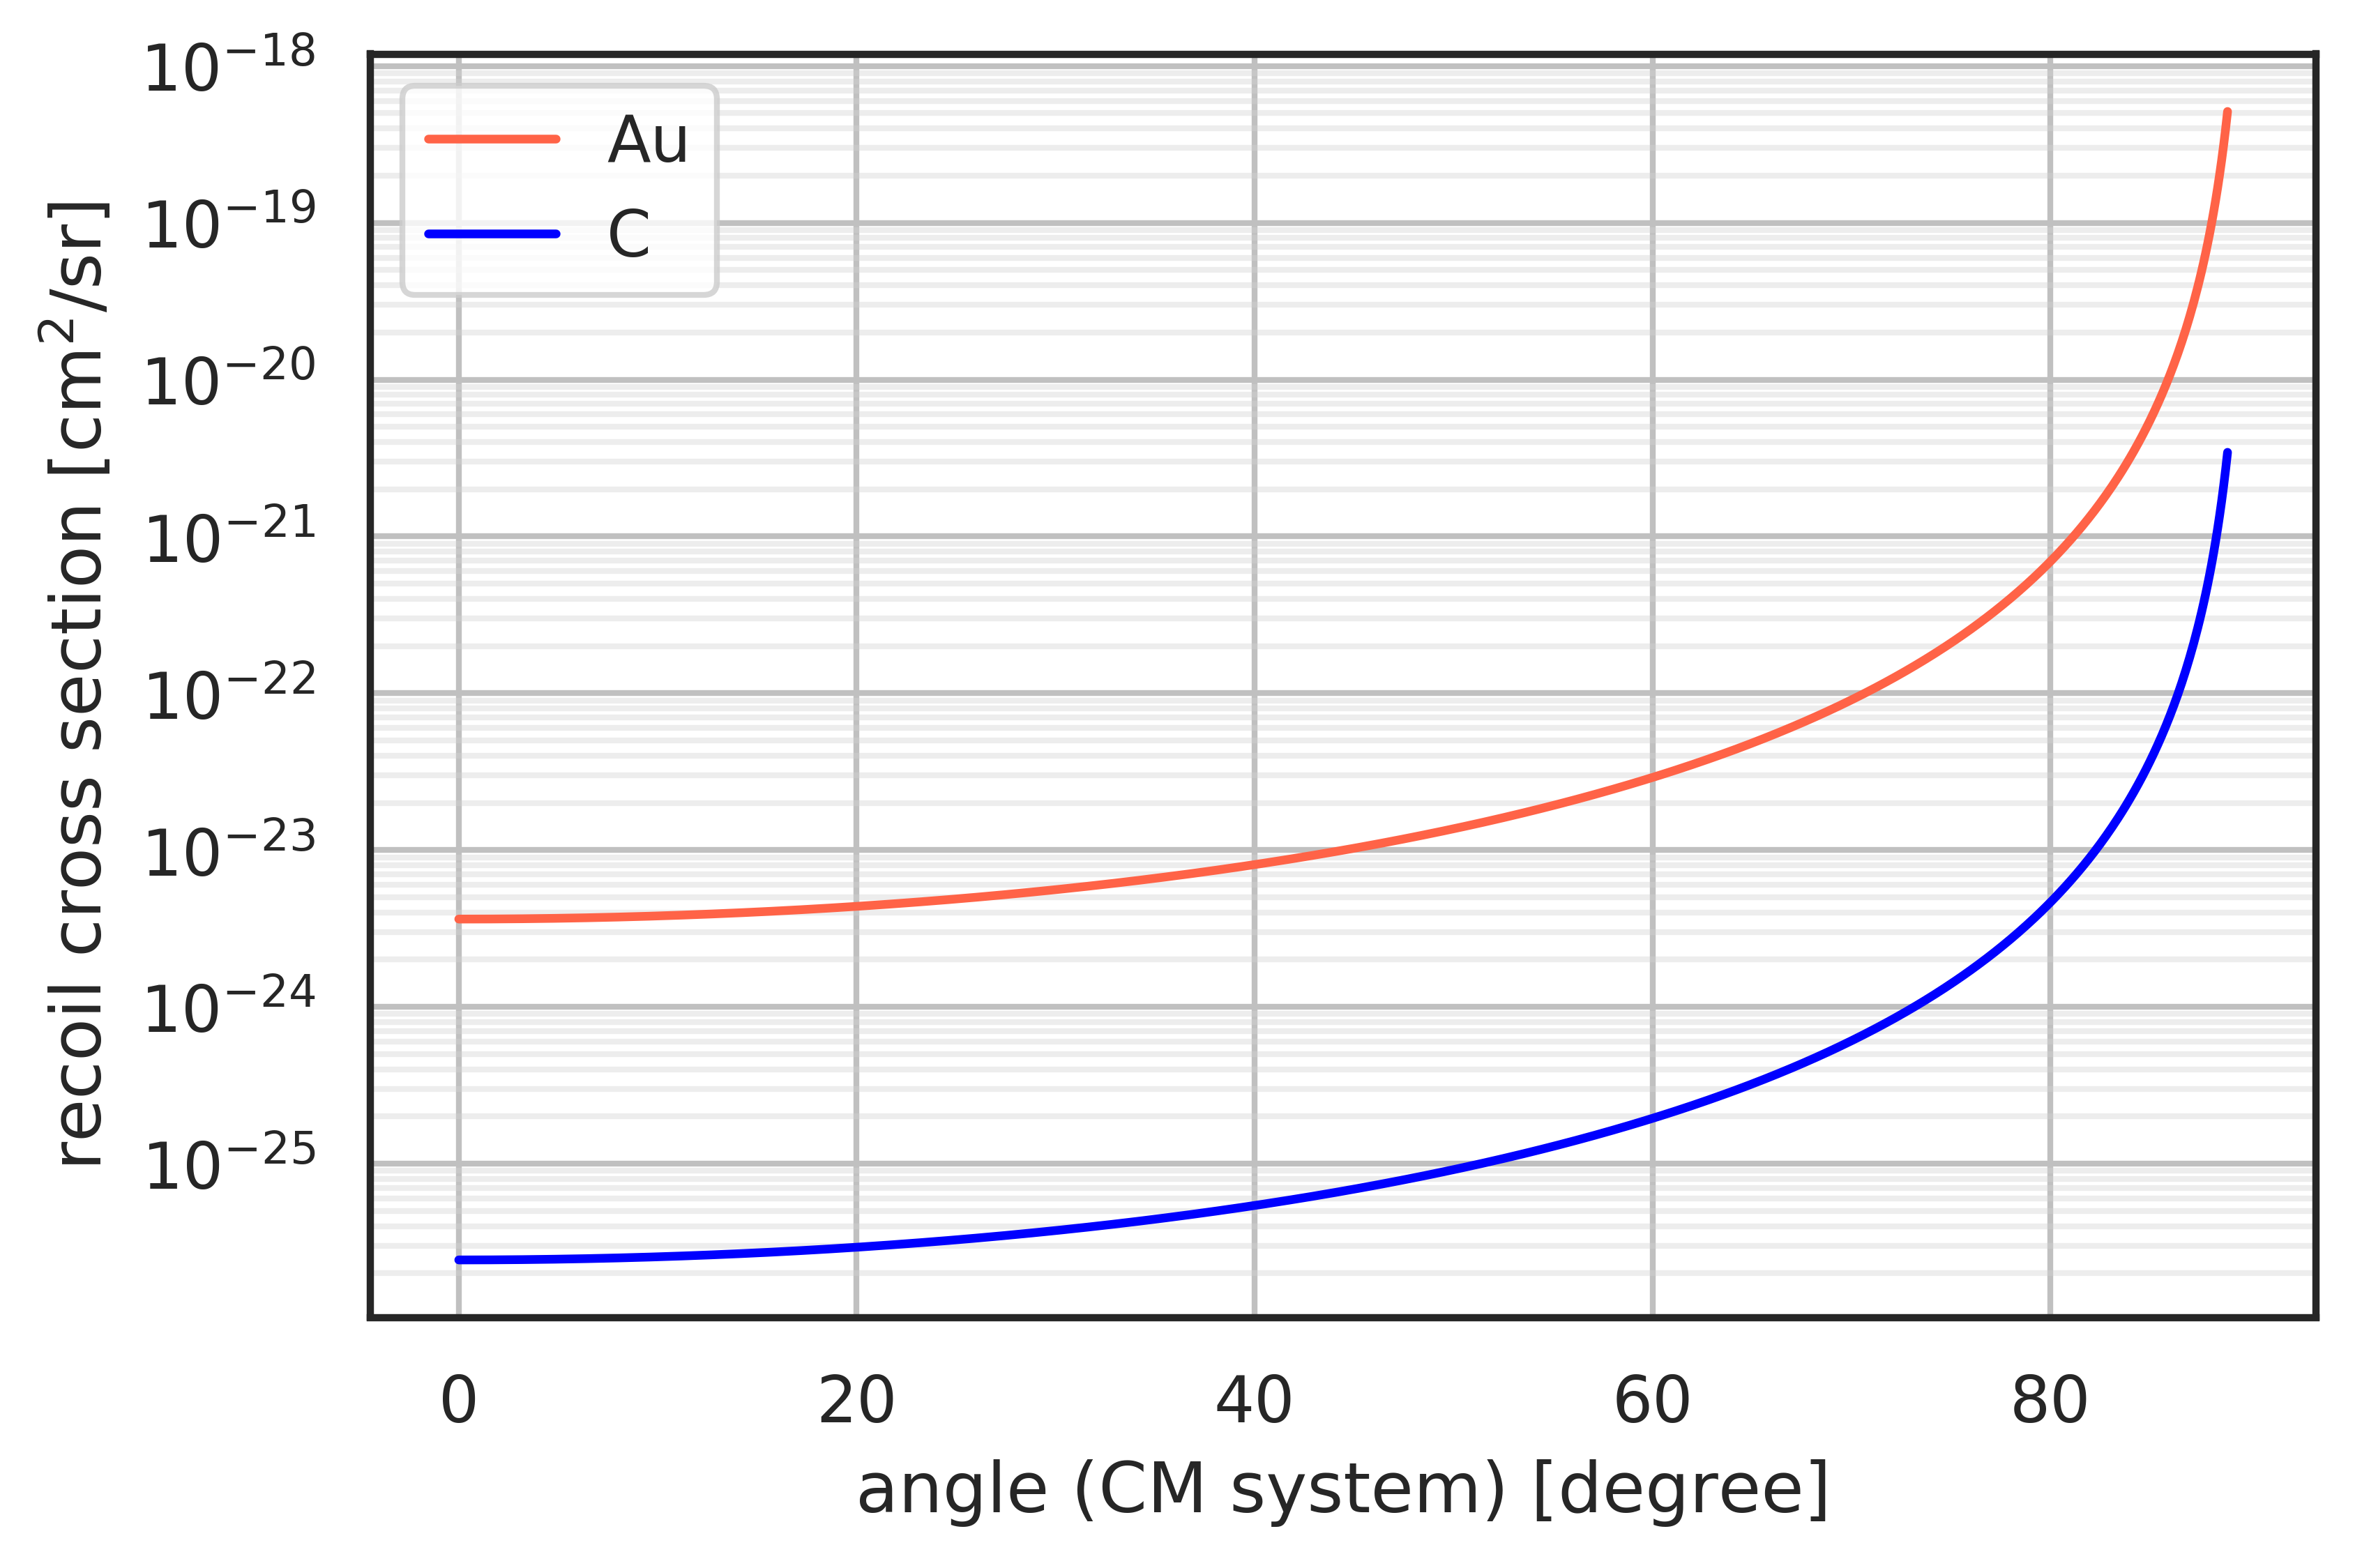
\includegraphics[width=110mm]{picture/cali/recoilcs.png}
\caption{微分反跳断面積の角度依存性}
\label{recoilcs}
\end{figure}
%図\ref{fig:recoil}から分かるように、反跳された原子核のエネルギーは炭素や金がターゲットのときは$E < 1  {\rm MeV}$となる。
%しかし、ピークはそれぞれの角度において1.7 MeV$\sim$1.9 MeVの間に見られた。一般に比電離は阻止能に比例するため、PINフォトダイオードの中で同じエネルギーの陽子に対してより多くの電子を電離させた可能性がある。

\vspace*{7mm}
以上のようにバックグラウンドの考察を行ったがいずれも根本的な解決には至っていない。散乱由来のものであるのか確認するために、ターゲットをなくした状態で計測を行うなどの工夫を行うことが改善点として挙げられる。

 %\vspace*{20mm}



\end{document}